\documentclass{article}
\usepackage{amsmath}
\usepackage{amsthm}
\usepackage{amssymb}
\usepackage{graphicx}

% Definitions / Theorems
%%%%%%%%%%%%%%%%%%%%%%
\newtheorem{definition}{Definition}
\newtheorem{thm}{Theorem}
%%%%%%%%%%%%%%%%%%%%%%

% Examples
%%%%%%%%%%%%%%%%%%%%%%
\newtheorem*{remark*}{Example}
\newtheorem*{definition*}{Meaning}
%%%%%%%%%%%%%%%%%%%%%%

% Misc
%%%%%%%%%%%%%%%%%%%%%%
\newtheorem{plain}{Symbol}
\newenvironment{problem}[2][Problem]{\begin{trivlist}
\item[\hskip \labelsep {\bfseries #1}\hskip \labelsep {\bfseries #2.}]}{\end{trivlist}}

%%%%%%%%%%%%%%%%%%%%%%

% Real Numbers
%%%%%%%%%%%%%%%%%%%%%%
\newcommand{\R}{\mathbb{R}}
\newcommand{\N}{\mathbb{N}}
%%%%%%%%%%%%%%%%%%%%%%

\title{Math\_226 Written Homework 2: Series}
\author{Randy Truong}
\begin{document}
\maketitle
\begin{problem}{1.1}
  Look at the following problems from 10.1: 22, 60, 108, 126
\end{problem}
\begin{problem}{1.1.1 (Problem 22)}
  Find a formula for the nth formula for the $n$th term
  of the sequence.
  \[ 2, 6, 10, 14, 18, \dots\]
\end{problem}
\[ \textrm{let} \{a_{n}\} = {2,6,10,14,18,...}\]
\[ \{a_{n}\}_{n=1} = 4n-2\]
\begin{problem}{1.1.2 (Problem 60)}
  Determine whether the sequence diverges or converges. If the
  sequence converges, find its limit.
  \[ \{a_{n}\} = \sqrt[n]{n^{2}}\]
  \[ \textrm{let}~ \{a_{n}\} = (n^{2})^{\frac{1}{n}}\]
  \[ a_{n} = e^{\ln(a_{n})}\]
  \[ \Rightarrow a_{n} = e^{\ln((n^{2})^{\frac{1}{n}})}\]
  \[ \Rightarrow a_{n} = e^{\frac{1}{n}\ln(n^{2})}\]
  \[ \textrm{let} ~ f(x) = e^{x}, ~ \textrm{let} ~ x(n) = \frac{1}{n}\ln({n^{2}})\]
  \[ \lim_{n \rightarrow \infty}\frac{\ln(n^{2})}{n} = \frac{\infty}{\infty} \]
  \begin{center}
    Because this is in indeterminate form, use L'Hopital's Rule
  \end{center}
  \[ \Rightarrow \frac{\frac{d}{dx} (\ln(n^{2}))}{\frac{d}{dx}(n)}\]
  \[ \Rightarrow \frac{\frac{1}{n^{2}} \cdot 2n}{1} = \frac{2}{n}\]
  \[ \Rightarrow \lim_{n \rightarrow \infty} \frac{2}{n} = 0 \]
  \begin{center}
    The sequence converges to 0.
  \end{center}

\end{problem}
\begin{problem}{1.1.3 (Problem 108)}
  Suppose the following recursive sequence converges,
  find its limit.
  \[ \sqrt{1},\sqrt{1+\sqrt{1}}, \sqrt{1+\sqrt{1+\sqrt{1}}}, \dots\]
\end{problem}
\textbf{Intuition.} Use the monotonic convergence theorem
\[ \textrm{let} ~ \{a_{n+1}\} ~ \textrm{be a recursive sequence}\]

\begin{center}
  Since $ 1 = \sqrt{1}$, we can let $ a_{1} = 1 $
  \[ \{ a_{n+1}\}_{a_{1} = 1} = \sqrt{1+a_{n}}\]
\end{center}
Given that we know that $ a_{n+1} $ converges, we are
able to assume that

\[ \textrm{Suppose} ~ \lim_{n \rightarrow \infty} a_{n} = L \]
\[ \{ a_{n+1}\}_{a_{1} = 1} = \sqrt{1+a_{n}}\]
\[ \Rightarrow L = \sqrt{1 + L}\]
\[ \Rightarrow L^{2} = 1 + L \]
\[ \Rightarrow L^{2} - L - 1 = 0 \]
\begin{center}
  Use the quadratic formula
\end{center}

\[ \Rightarrow \frac{-b \pm \sqrt{b^{2}-4ac}}{2a} = \frac{1 \pm \sqrt{1+4}}{2(1)} = \frac{1 \pm \sqrt{5}}{2}\]

Since we know that all terms $ a_{n+1}$ are positive, we know
that the limit $ L $ is
\[ L = \lim_{n \rightarrow \infty} a_{n+1} =  \frac{1 + \sqrt{5}}{2}\]





\begin{problem}{1.1.4 (Problem 126)}
  Determine if the following sequence converges or diverges. If
  the sequence converges, find its limit.
  \[ \{a_{n}\} = n - \frac{1}{n}\]
  \[ \Rightarrow \lim_{n \rightarrow \infty} a_{n} = \lim_{n \rightarrow \infty} \Biggr(n-\frac{1}{n}\Biggr)\]
  \[ \Rightarrow \lim_{n \rightarrow \infty} n - \lim_{n \rightarrow \infty } \frac{1}{n}\]
  \[ \Rightarrow \infty - 0 \]
  \[ \Rightarrow \infty \]
  \begin{center}
    The sequence does not converge and therefore diverges.
  \end{center}

\end{problem}

\begin{problem}{2.1}
  Determine whether the following series converges or diverges,
  and show that your answers are correct by citing (with full
  justification) the appropriate definitions or theorems.
\end{problem}
\begin{problem}{2.1.1}
  \[ \sum_{n=1}^{\infty}\frac{1}{\sqrt{2n}-\sin^{2}{n}}\]
\end{problem}
\begin{problem}{2.1.2}
  \[ 1 + \frac{3}{4} + \frac{4}{6} + \frac{5}{8} + \frac{6}{10} +
  \frac{7}{12} + \dots \]
\end{problem}
\begin{problem}{2.1.3}
  \[ \sum_{n=2}^{\infty}\frac{1}{n(ln(n))^{2}}\]
\end{problem}
\begin{problem}{3.1}
  Take the following as \textit{fact}: a ball dropped from a height
  $ H $ meters takes $ \sqrt{H/5}$ seconds to hit the ground.
  (Likewise, a ball launched from the ground to a maximum height
  $ H$ takes $ \sqrt{H/5}$ seconds to reach tis peak.) Using this,
  determine the total time taken for the infinite processin Example 3 of 10.2.
\end{problem}
\newpage
\begin{problem}{4.1}
  \begin{figure}

    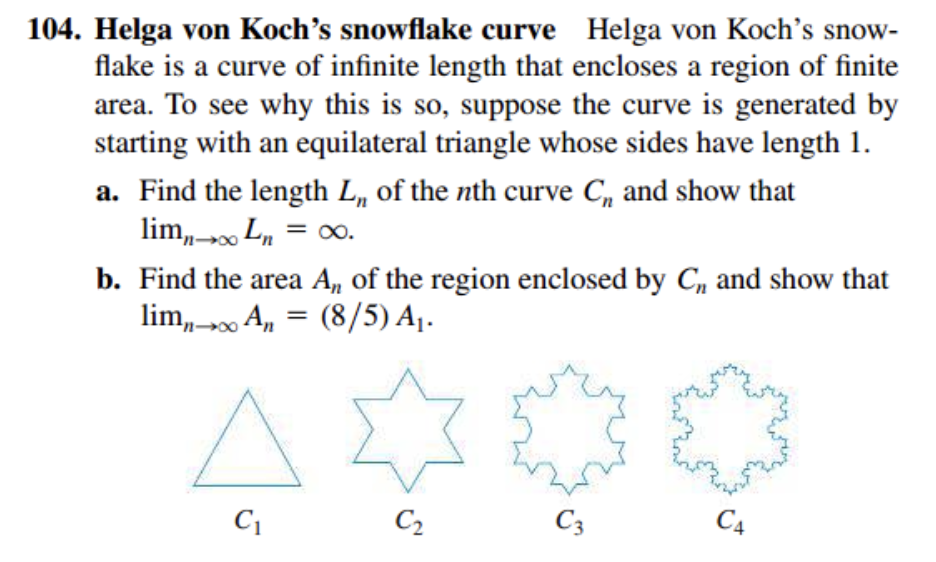
\includegraphics[width=0.85\linewidth]{problem.png}
  \end{figure}

\end{problem}

\begin{problem}{5.1}
  Determine all values of $ p $ for which the following series
  converges using the Integral Test. Make sure you justify
  why the intergral test is applicable
  \[ \sum_{n=3}^{\infty}\frac{1}{n(ln(n))^{p+2}}\]
\end{problem}
\begin{problem}{6.1}
  Give a value of $ n $ for which the expression
  \[ \sum_{k=1}^{\infty}\frac{1}{k^{3}}\]
  is within $ 0.001 $ of its exact value. Justify your claim.
\end{problem}
\end{document}
